\documentclass[10.5pt,scale=1.0,t,aspectratio=169,hyperref={pdfpagelabels=false}]{beamer}
\usepackage{lipsum}
\usepackage{color}
\usepackage{amsfonts}
\usepackage{amsmath,mathtools}
\usepackage{mathrsfs}
\usepackage{array}
\usepackage{algorithm}
\usepackage{hyperref}
\usepackage[spanish,es-nodecimaldot]{babel}
\usepackage[utf8]{inputenc}
\usepackage{graphicx}
\usepackage{multicol}
\usepackage{multirow}
\usepackage{enumitem}
\usepackage[document]{ragged2e}
\usepackage[absolute,overlay]{textpos}
\textblockorigin{0mm}{0mm} 
\usefonttheme[onlymath]{serif}
\usepackage{verbatim}
\usepackage{cite}
\usepackage{multicol}




\newenvironment{conditions}[1][where:]
{#1 \begin{tabular}[t]{>{$}l<{$} @{${}={}$} l}}
	{\end{tabular}\\[\belowdisplayskip]}


\newcolumntype{L}{>{$}l<{$}} % math-mode version of "l" column type


\newcounter{saveenumi}
\newcommand{\seti}{\setcounter{saveenumi}{\value{enumi}}}
\newcommand{\conti}{\setcounter{enumi}{\value{saveenumi}}}

\setbeamertemplate{bibliography item}{\insertbiblabel}


\hypersetup{colorlinks=true,
	linkcolor=blue,
	linktoc=all,				
	citecolor=blue,
	urlcolor=red,
	pdftitle={FUNDAMENTOS DE AUTOMATIZACIÓN Y CONTROL},
	pdfauthor={Santiago Rúa Pérez},
	pdfcreator={Santiago Rúa Pérez}}


\definecolor{GreenDark}{rgb}{0.0, 0.60, 0.0}
\definecolor{RedDark}{rgb}{183, 0.0, 0.0}
\definecolor{BlueDark}{rgb}{0.0, 0.0, 167}
\definecolor{BlueLight}{rgb}{0.2, 0.451, 0.517}


\graphicspath{{imag/}}

\newcommand{\Ho}{$H_{0}$}
\newcommand{\Ha}{$H_{a}$}
\newcommand{\Nota}{{\bf Nota: }}
\newcolumntype{P}[1]{>{\centering\arraybackslash}p{#1}}
\newcolumntype{M}[1]{>{\centering\arraybackslash}m{#1}}

\newcommand{\less}{<}
\newcommand{\greater}{>}


\setlength{\parindent}{1em}
\setlength{\parskip}{.6em}
\renewcommand{\baselinestretch}{.9}

%%%%    C environment    ---------------- %%%%%%%%%%%%%%%.
\usepackage{listings}
\usepackage{xcolor}
\definecolor{mGreen}{rgb}{0,0.6,0}
\definecolor{mGray}{rgb}{0.5,0.5,0.5}
\definecolor{mPurple}{rgb}{0.58,0,0.82}
\definecolor{backgroundColour}{rgb}{0.95,0.95,0.92}

\lstdefinestyle{CStyle}{
	backgroundcolor=\color{backgroundColour},   
	commentstyle=\color{mGreen},
	keywordstyle=\color{magenta},
	numberstyle=\tiny\color{mGray},
	stringstyle=\color{mPurple},
	basicstyle=\scriptsize,
	breakatwhitespace=false,         
	breaklines=true,                 
	captionpos=b,                    
	keepspaces=true,                 
	numbers=left,                    
	numbersep=5pt,                  
	showspaces=false,                
	showstringspaces=false,
	showtabs=false,                  
	tabsize=2,
	language=C
}
%%--------------------------------------------------------------------------


\title{Electrónica Digital II}   
\author{Santiago Rúa Pérez, PhD.} 
\date{\today} 

\setlength{\TPHorizModule}{\textwidth}
\setlength{\TPVertModule}{\textwidth}

\newcommand{\btVFill}{\vskip0pt plus 1filll}


\setbeamertemplate{sidebar right}{}
\setbeamertemplate{footline}
{
	\leavevmode%
	\hbox{%
		\begin{beamercolorbox}[wd=.333333\paperwidth,ht=2.25ex,dp=1ex,center]{author in head/foot}%
			\usebeamerfont{author in head/foot}\insertshortauthor
		\end{beamercolorbox}%
		\begin{beamercolorbox}[wd=.333333\paperwidth,ht=2.25ex,dp=1ex,center]{title in head/foot}%
			\usebeamerfont{title in head/foot}\insertshorttitle
	\end{beamercolorbox}}%
	\vskip0pt%
}
\makeatother

\begin{document}
	%%%%%%%%%%%%%%%%%% FRAME %%%%%%%%%%%%%%%%%%%%%%%%%%
	\begin{frame}
		\titlepage
	\end{frame}
	%%%%%%%%%%%%%%%%% FRAME START %%%%%%%%%%%%%%%%%%%%%%%%%%
	\frame{
		%\frametitle{}
		\begin{center}
			\LARGE \textcolor{blue}{INTRODUCCIÓN A LOS MICROCONTROLADORES}
		\end{center}
		
	}
	
	%%%%%%%%%%%%%%%%% FRAME %%%%%%%%%%%%%%%%%%%%%%%%%%

%%%%%%%%%%%%%%%%% FRAME %%%%%%%%%%%%%%%%%%%%%%%%%%
\begin{frame}
\frametitle{Objetivos}
\begin{itemize}
\item Entender la estructura de funcionamiento de un microcontrolador.
\item Entender como se traduce un programa de C a ejecución en el microcontrolador.
\item Entender la diferencia en Hardvard y Von Neumann.
\end{itemize}
\end{frame}
%%%%%%%%%%%%%%%%% FRAME %%%%%%%%%%%%%%%%%%%%%%%%%%
\begin{frame}
	\frametitle{Lenguaje C a lenguaje de máquina}
	\begin{figure}
		\centering
		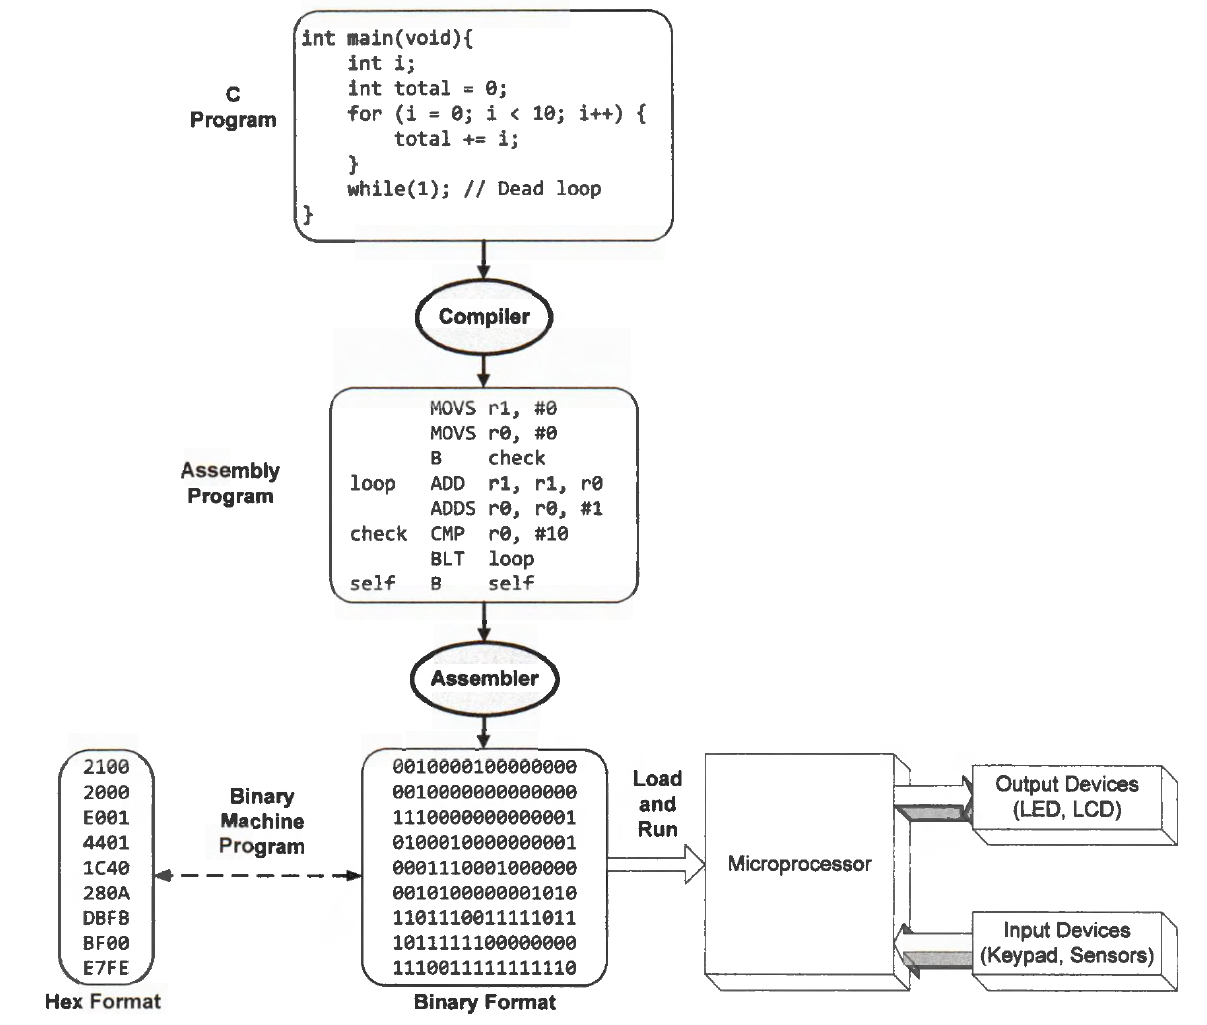
\includegraphics[scale=0.4]{LenguajeCMicros}
	\end{figure}
\end{frame}
%%%%%%%%%%%%%%%%% FRAME %%%%%%%%%%%%%%%%%%%%%%%%%%
\begin{frame}
	\frametitle{Hardware vs Von Neumann}
		
	\begin{columns}
		\column{0.5\linewidth}
		\textcolor{blue}{Hardvard}
		\begin{figure}
			\centering
			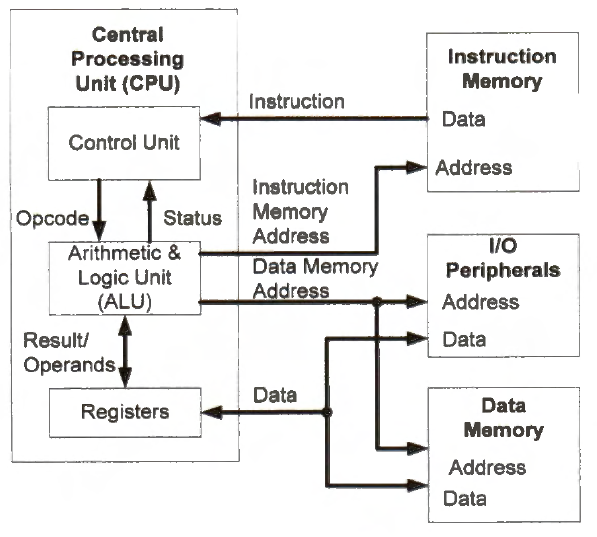
\includegraphics[scale=0.5]{Harvard}
		\end{figure}
	
		\column{0.5\linewidth}
		\textcolor{blue}{Von Neumann}
		\begin{figure}
			\centering
			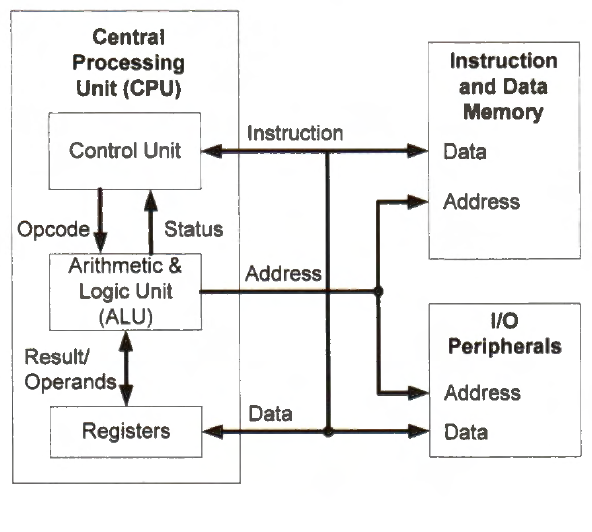
\includegraphics[scale=0.5]{VonNeumann}
		\end{figure}
	\end{columns}
\end{frame}

%%%%%%%%%%%%%%%%% FRAME %%%%%%%%%%%%%%%%%%%%%%%%%%
\begin{frame}
	\frametitle{Tarjeta a trabajar}
	\begin{columns}
		\column{0.5\linewidth}
		\begin{itemize}
			\item Procesador Cortex M4 de 32-bit
			\item Freescale Kinetis MK64FN1M0VLL12 
			\begin{itemize}
				\item 120 Mhz max clock, 1 MB flash, 256 kB RAM
				\item Bajo consumo.
				\item Cantidad grande de periféricos. 
			\end{itemize}
			\item Costo 47USD (Digikey)
			\item Perifericos externos: led RGB, acelerometro y magnetómetro (FXOS8700CQ), dos pulsadores, SD, Ethernet
			\item Compatible con los pines de arduino.
			\item mbed.org habilitado 
		\end{itemize}
		
		\column{0.5\linewidth}
		\begin{figure}
			\centering
			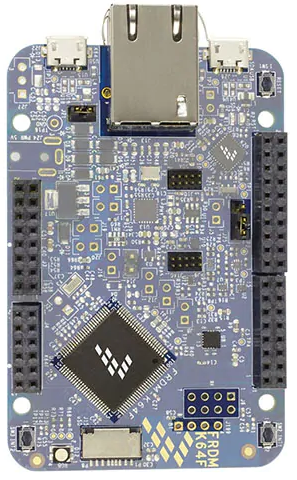
\includegraphics[scale=0.5]{FRDMK64F}
		\end{figure}
	\end{columns}
\end{frame}

%%%%%%%%%%%%%%%%% FRAME %%%%%%%%%%%%%%%%%%%%%%%%%%
\begin{frame}
	\frametitle{Tarjeta a trabajar}
	\begin{columns}
		\column{0.5\linewidth}
		\begin{itemize}
			\item Procesador Cortex M4 de 32-bit
			\item Freescale Kinetis MK64FN1M0VLL12 
			\begin{itemize}
				\item 120 Mhz max clock, 1 MB flash, 256 kB RAM
				\item Bajo consumo.
				\item Cantidad grande de periféricos. 
			\end{itemize}
			\item Costo 47USD (Digikey)
			\item Perifericos externos: led RGB, acelerometro y magnetómetro (FXOS8700CQ), dos pulsadores, SD, Ethernet
			\item Compatible con los pines de arduino.
			\item mbed.org habilitado 
		\end{itemize}
		
		\column{0.5\linewidth}
		\begin{figure}
			\centering
			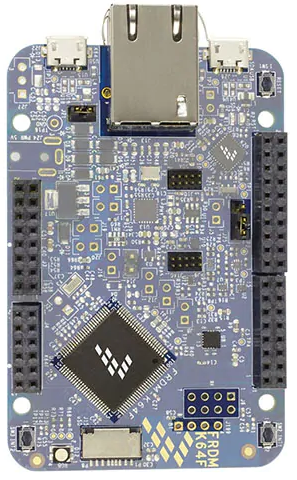
\includegraphics[scale=0.5]{FRDMK64F}
		\end{figure}
	\end{columns}
\end{frame}

%%%%%%%%%%%%%%%%% FRAME %%%%%%%%%%%%%%%%%%%%%%%%%%
\begin{frame}
	\frametitle{Tarjeta a trabajar}
		\begin{figure}
			\centering
			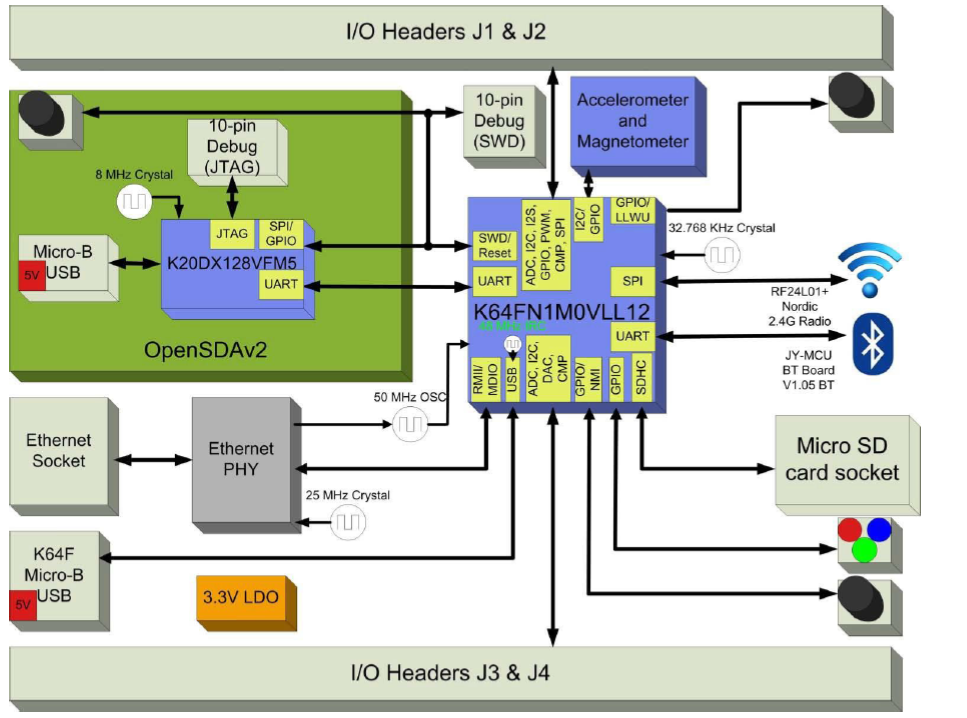
\includegraphics[scale=0.4]{FRDMK64RMI}
		\end{figure}
\end{frame}

%%%%%%%%%%%%%%%%% FRAME %%%%%%%%%%%%%%%%%%%%%%%%%%
\begin{frame}
	\frametitle{Documentos Importantes}
	\begin{itemize}
		\item \href{https://www.nxp.com/products/processors-and-microcontrollers/arm-microcontrollers/general-purpose-mcus/k-series-cortex-m4/k6x-ethernet/kinetis-k64-120-mhz-256-kb-sram-microcontrollers-mcus-based-on-arm-cortex-m4-core:K64_120?tab=Documentation_Tab}{Kinetis K64: 120MHz Cortex-M4F up to 1MB Flash 100-144pin }. Necesario para revisar todos los registros y capacidades del procesador. 
		\item \href{https://www.nxp.com/design/development-boards/freedom-development-boards/mcu-boards/freedom-development-platform-for-kinetis-k64-k63-and-k24-mcus:FRDM-K64F}{FRDMK64FUG, FRDM-K64F Freedom Module User’s Guide}. Necesario para revisar las capacidades y conexiones de la tarjeta FRDMK64F.
		\item \href{https://www.nxp.com/design/development-boards/freedom-development-boards/mcu-boards/freedom-development-platform-for-kinetis-k64-k63-and-k24-mcus:FRDM-K64F}{FRDMK64 Schematic}. Necesario para revisar las conexiones físicas del sistemas.
		\item \href{https://www.nxp.com/document/guide/get-started-with-the-frdm-k64f:NGS-FRDM-K64F}{Get Started}. Guia de inicio para probar la tarjeta de desarrollo. Hacerlo y validarlo inmediatamente. 
	\end{itemize}
	
\end{frame}

%%%%%%%%%%%%%%%%% FRAME %%%%%%%%%%%%%%%%%%%%%%%%%%
\begin{frame}
	\frametitle{Kinetis K60}
		\begin{figure}
			\centering
			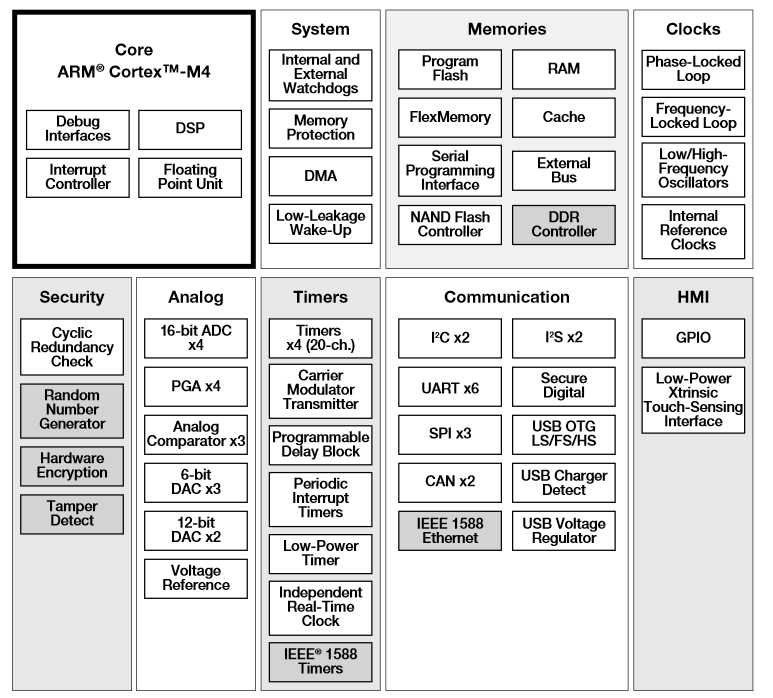
\includegraphics[scale=0.6]{KinetisK60}
		\end{figure}
\end{frame}
%%%%%%%%%%%%%%%%% FRAME %%%%%%%%%%%%%%%%%%%%%%%%%%
\begin{frame}
	\frametitle{Comparing ARM}
	\begin{figure}
		\centering
		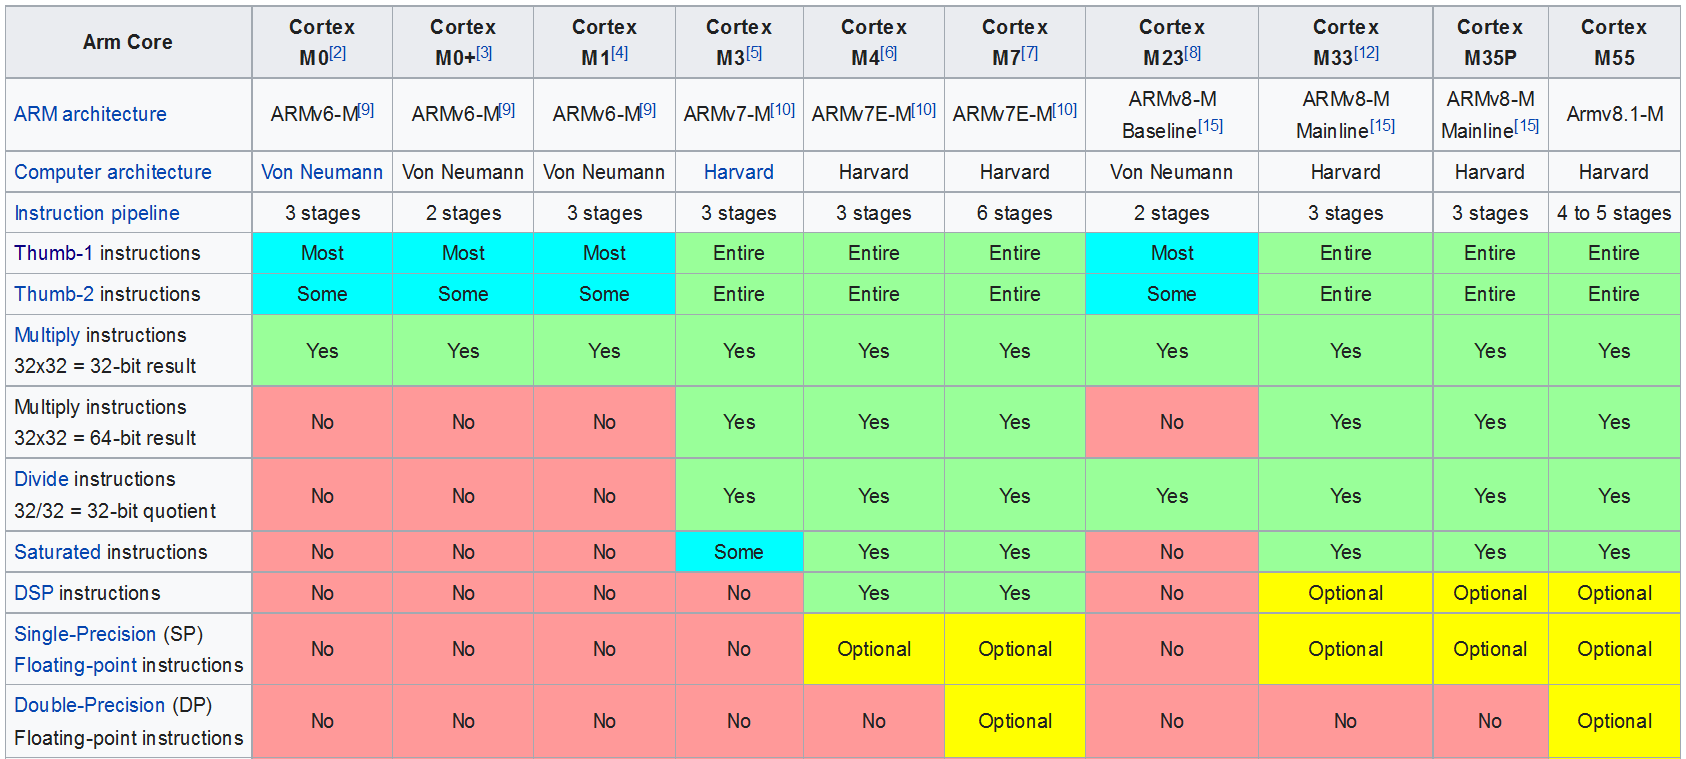
\includegraphics[scale=0.3]{ComparingARM}
	\end{figure}
\end{frame}
%%%%%%%%%%%%%%%%% FRAME %%%%%%%%%%%%%%%%%%%%%%%%%%
\begin{frame}
	\frametitle{Ejecutando programa en arquitectura Cortex M}
	\begin{figure}
		\centering
		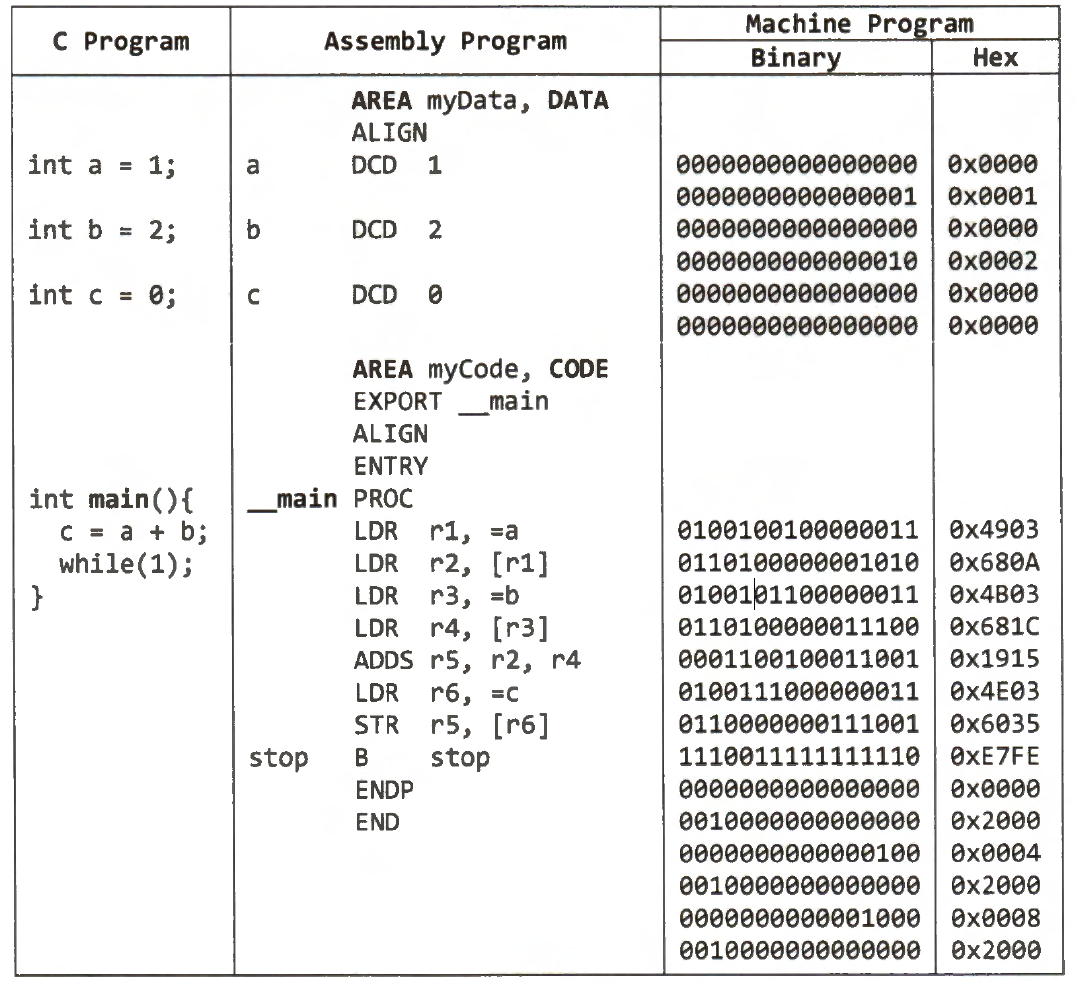
\includegraphics[scale=0.4]{EjecutandoPrograma}
	\end{figure}
\end{frame}

%%%%%%%%%%%%%%%%% FRAME %%%%%%%%%%%%%%%%%%%%%%%%%%
\begin{frame}
	\frametitle{Arquitectura Cortex M-4}
	\begin{figure}
		\centering
		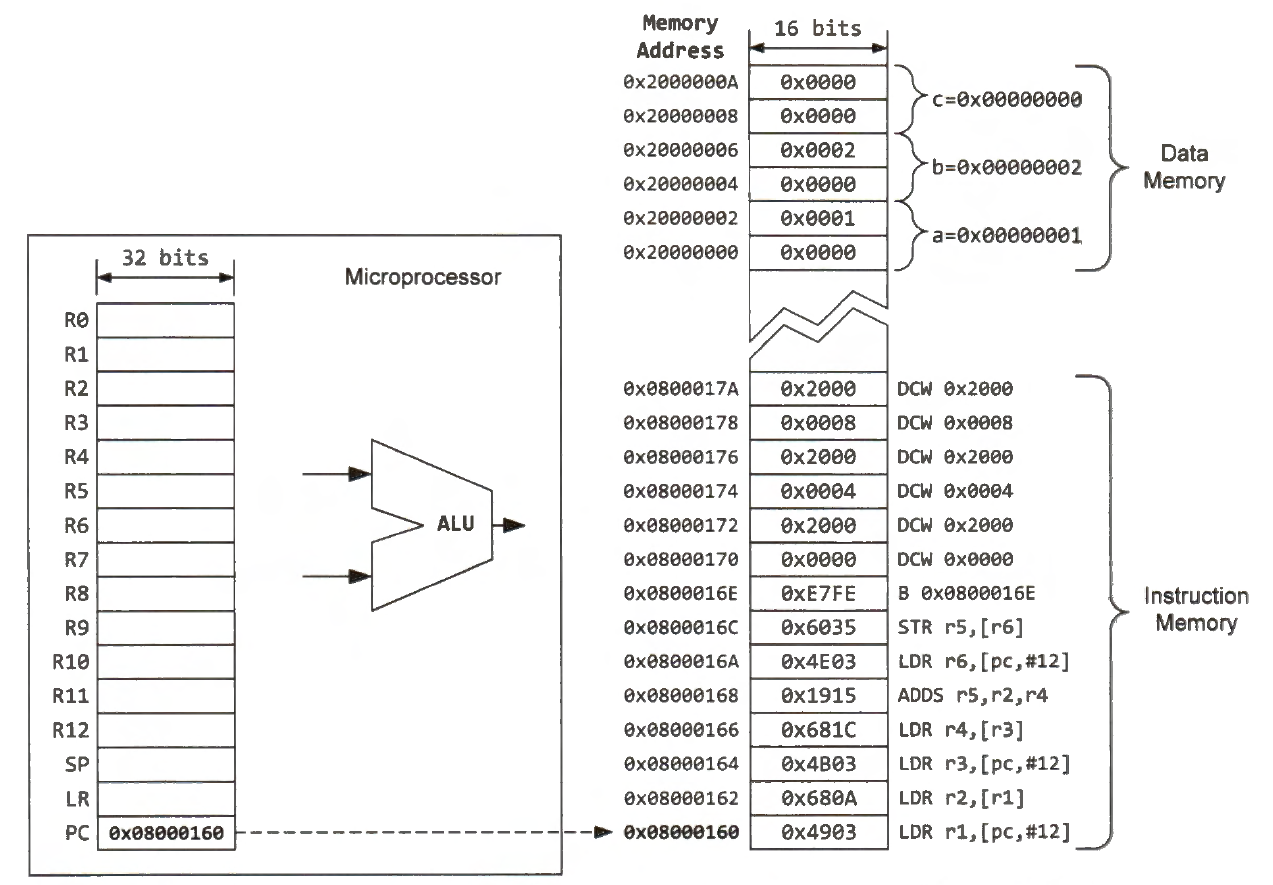
\includegraphics[scale=0.45]{ArquitecturaARM}
	\end{figure}
\end{frame}

%%%%%%%%%%%%%%%%% FRAME %%%%%%%%%%%%%%%%%%%%%%%%%%
\begin{frame}
	\frametitle{Arquitectura Cortex M-4}
	\textbf{Dirección} -- \textbf{Instrucción de ensamblador} -- \textbf{Resultado}.
	\begin{itemize}
		\item 0x08000160 --- LDR r1, [pc, \#12] --- r1 = 0x2000000.
		
		{\small Carga la direccion de memoria de la variable global a en el registro r1.}
		
		\item 0x08000162 --- LDR r2, [r1] --- r2 = 0x00000001.
		
		{\small Carga el valor de la variable global a al registro r2.}
		
		\item 0x08000164 --- LDR r3, [pc, \#12] --- r3 = 0x20000004.
		
		{\small Carga la direccion de memoria de la variable global b en el registro r3}
		
		\item 0x08000166 --- LDR r4, [r3] --- r4 = 0x00000002.
		
		{\small Carga el valor de la variable global b al registro r4.}
		
		\item 0x08000168 --- ADDS r5, r2, r4 --- r5 = 0x00000003.
		
		{\small Suma el valor de a y b}
	\end{itemize}
\end{frame}
%%%%%%%%%%%%%%%%% FRAME %%%%%%%%%%%%%%%%%%%%%%%%%%
\begin{frame}
	\frametitle{Arquitectura Cortex M-4}
	\textbf{Dirección} -- \textbf{Instrucción de ensamblador} -- \textbf{Resultado}.
	\begin{itemize}
		\item 0x0800016A --- LDR r6, [pc, \#12] --- r6 = 0x20000008.
		
		{\small Carga la direccion de memoria de la variable global c en el registro r6.}
		
		\item 0x0800016C --- STR r5, [r6] --- mem[0x20000008] = 0x00000003.
		
		{\small Guarda la suma en la memoria de datos}
	
		\item 0x0800016E --- B 0x0800016E --- PC = 0x0800016E.
		
		{\small A punta a la direccion de memoria de sis mismo}
	\end{itemize}
\end{frame}

%%%%%%%%%%%%%%%%% FRAME %%%%%%%%%%%%%%%%%%%%%%%%%%
\begin{frame}
	\frametitle{Requerimientos de memoria}
		\begin{columns}
		\column{0.5\linewidth}
	 	\begin{itemize}
	 		\item Que se requiere almacenar en la memoria?
	 		\begin{itemize}
	 			\item Código
	 			\item Datos estáticos de solo lectura
	 			\item Datos estáticos de escritura
	 			\item Heap y el Stack
	 		\end{itemize}
 			\item Puede cambiar la información almacenada?
 			\begin{itemize}
 				\item No? Ponerla en memoria no volatil, solo lectura, usar const. Ej: instrucciones, contantes, valores iniciales.
 				\item Si? Ponerla en memoria de escritura y lectura. Ej: variables, resultados intermedios, direcciones de retorno. 
 			\end{itemize}
	 	\end{itemize}
		
		\column{0.5\linewidth}
		\begin{itemize}
			\item Cuanto tiempo que existir el dato?
			\begin{itemize}
				\item Reutilizar memoria desde que se pueda. 
			\end{itemize}
		\end{itemize}
	\end{columns}
\end{frame}

%%%%%%%%%%%%%%%%% FRAME %%%%%%%%%%%%%%%%%%%%%%%%%%
%%%%%%%%%%%%%%%%% FRAME %%%%%%%%%%%%%%%%%%%%%%%%%%
\begin{frame}
	\frametitle{Requerimientos de memoria}
	\begin{figure}
		\centering
		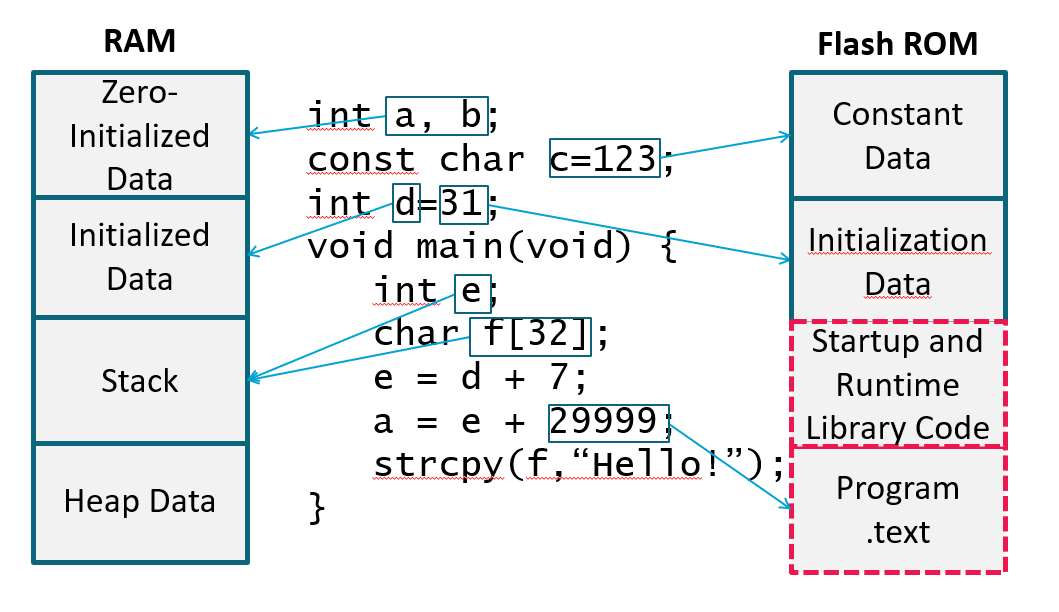
\includegraphics[scale=0.45]{ExampleMemory}
	\end{figure}
\end{frame}

%%%%%%%%%%%%%%%%% FRAME %%%%%%%%%%%%%%%%%%%%%%%%%%
\begin{frame}
	\frametitle{Calificadores para las variables}
	\begin{itemize}
		\item Modificar la declaración de las variables posibilita hacer entender al compilador el comportamiento que queremos.
		\item Contantes: nunca escritas o modificadas por el programa, almacenandolas en ROM y no RAM.
		\item Volatil: pueden cambiar por fuera del scope del programa, por ejemplo una interrupcion, entre otros. El compilador no debe realizar optimizaciones sobre este tipo de variables.
		\item Estaticas: declaradas o usadas dentro de las funciones, para retener valores de llamado a las mismas. Solo tienen alcance dentro de la función.
	\end{itemize}
\end{frame}
%%%%%%%%%%%%%%%%% FRAME %%%%%%%%%%%%%%%%%%%%%%%%%%
\begin{frame}
	\frametitle{Pila de llamado a funciones}
	\begin{figure}
		\centering
		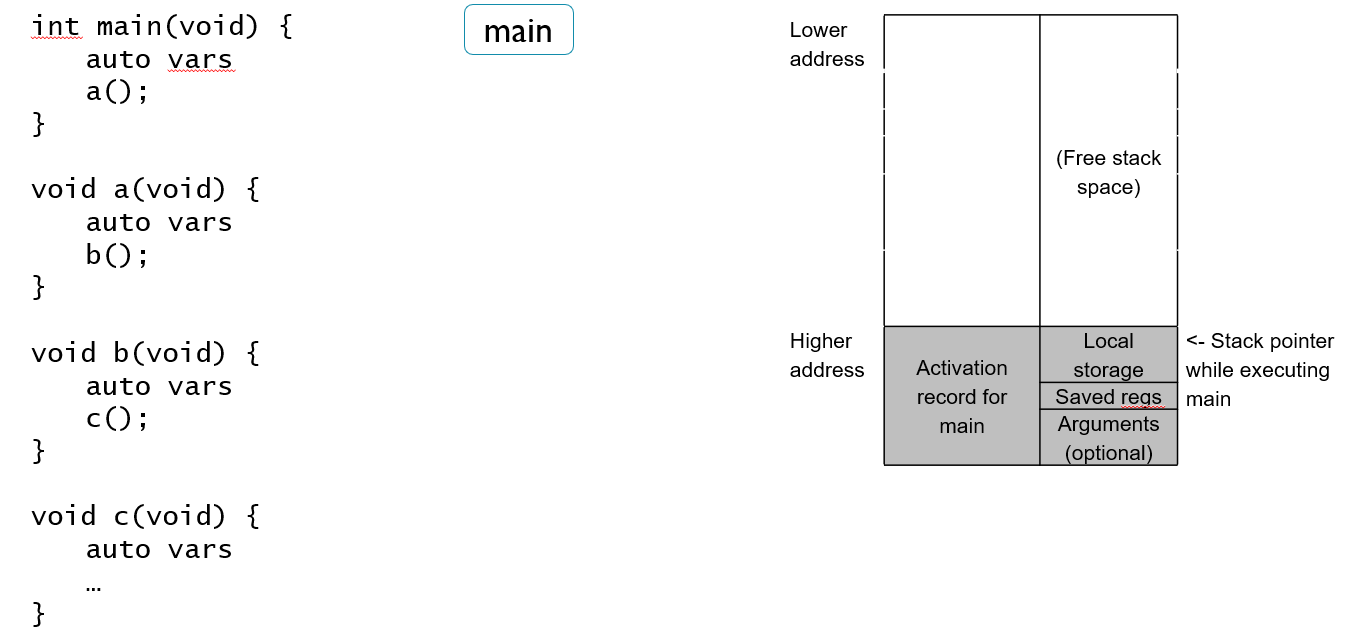
\includegraphics[scale=0.4]{StackFunction1}
	\end{figure}
\end{frame}
%%%%%%%%%%%%%%%%% FRAME %%%%%%%%%%%%%%%%%%%%%%%%%%
\begin{frame}
	\frametitle{Pila de llamado a funciones}
	\begin{figure}
		\centering
		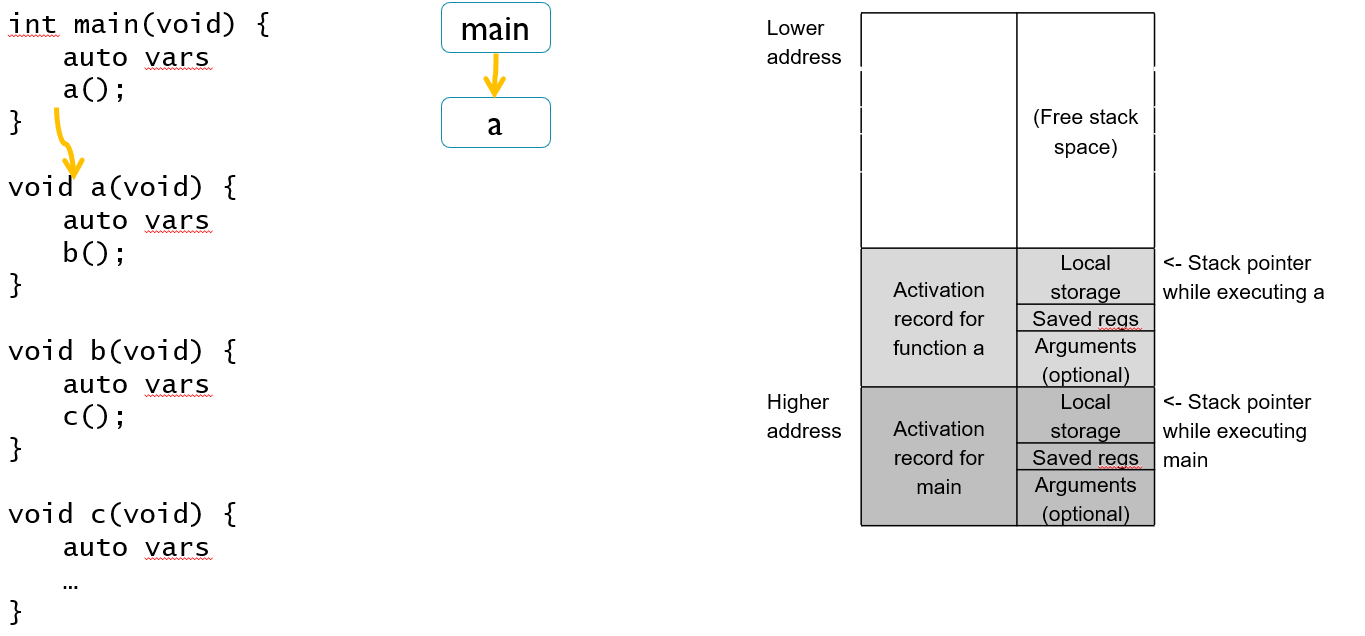
\includegraphics[scale=0.4]{StackFunction2}
	\end{figure}
\end{frame}
%%%%%%%%%%%%%%%%% FRAME %%%%%%%%%%%%%%%%%%%%%%%%%%
\begin{frame}
	\frametitle{Pila de llamado a funciones}
	\begin{figure}
		\centering
		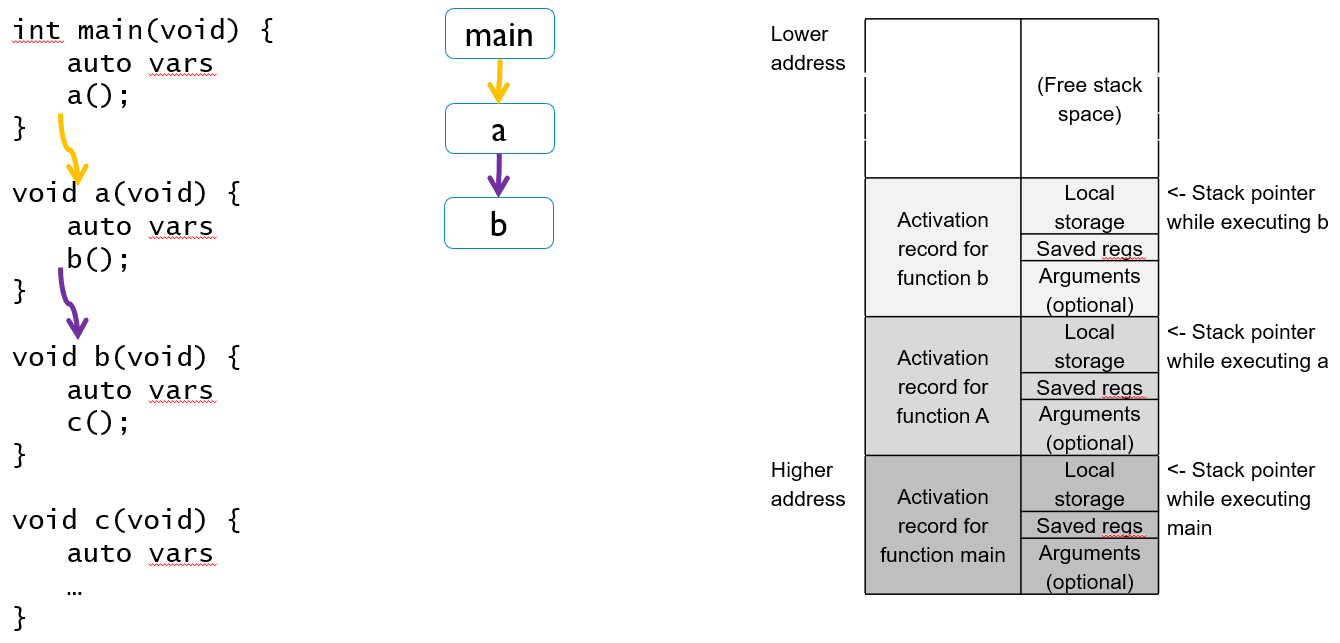
\includegraphics[scale=0.4]{StackFunction3}
	\end{figure}
\end{frame}
%%%%%%%%%%%%%%%%% FRAME %%%%%%%%%%%%%%%%%%%%%%%%%%
\begin{frame}
	\frametitle{Pila de llamado a funciones}
	\begin{figure}
		\centering
		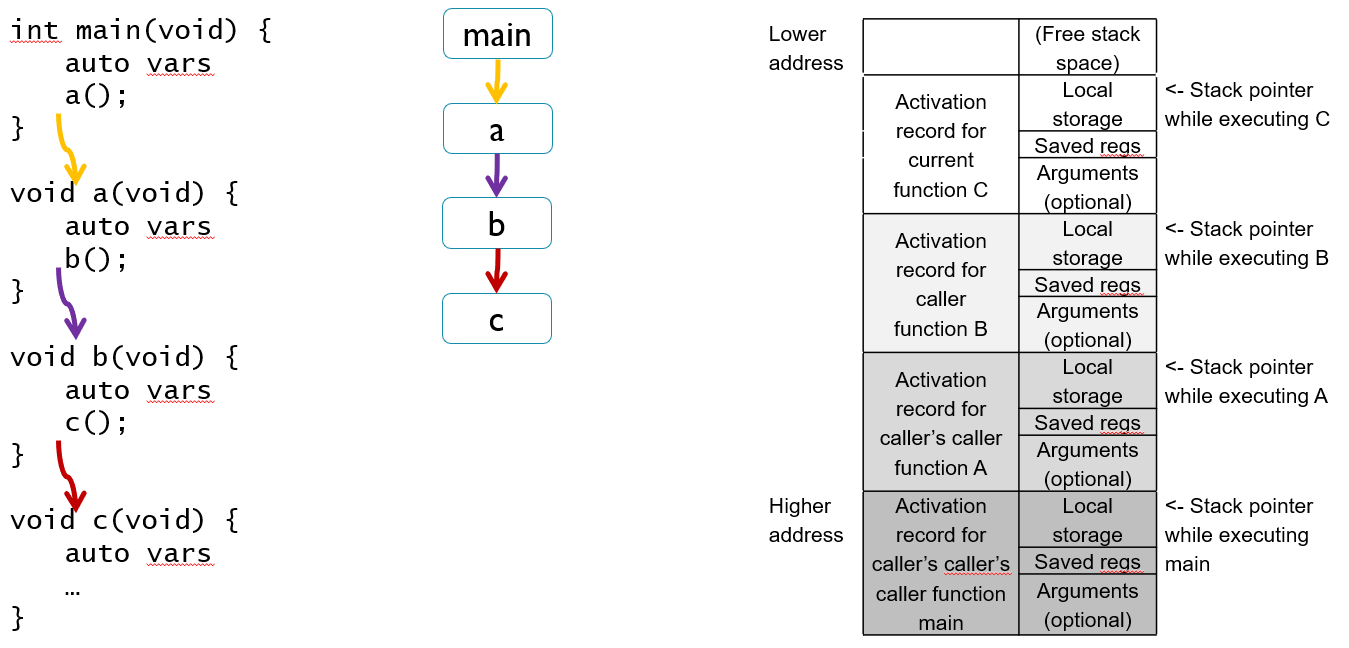
\includegraphics[scale=0.4]{StackFunction4}
	\end{figure}
\end{frame}
%%%%%%%%%%%%%%%%% FRAME %%%%%%%%%%%%%%%%%%%%%%%%%%
\begin{frame}
	\frametitle{Pila de llamado a funciones}
	\begin{figure}
		\centering
		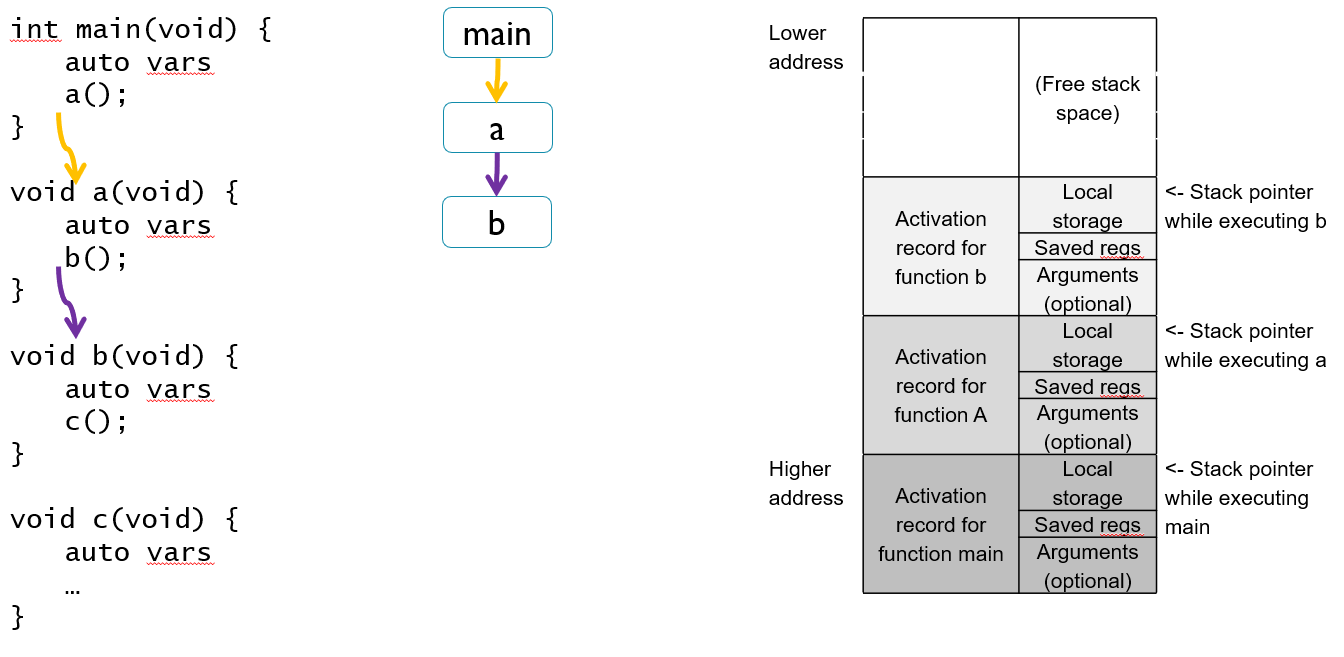
\includegraphics[scale=0.4]{StackFunction5}
	\end{figure}
\end{frame}
%%%%%%%%%%%%%%%%% FRAME %%%%%%%%%%%%%%%%%%%%%%%%%%
\begin{frame}
	\frametitle{Pila de llamado a funciones}
	\begin{figure}
		\centering
		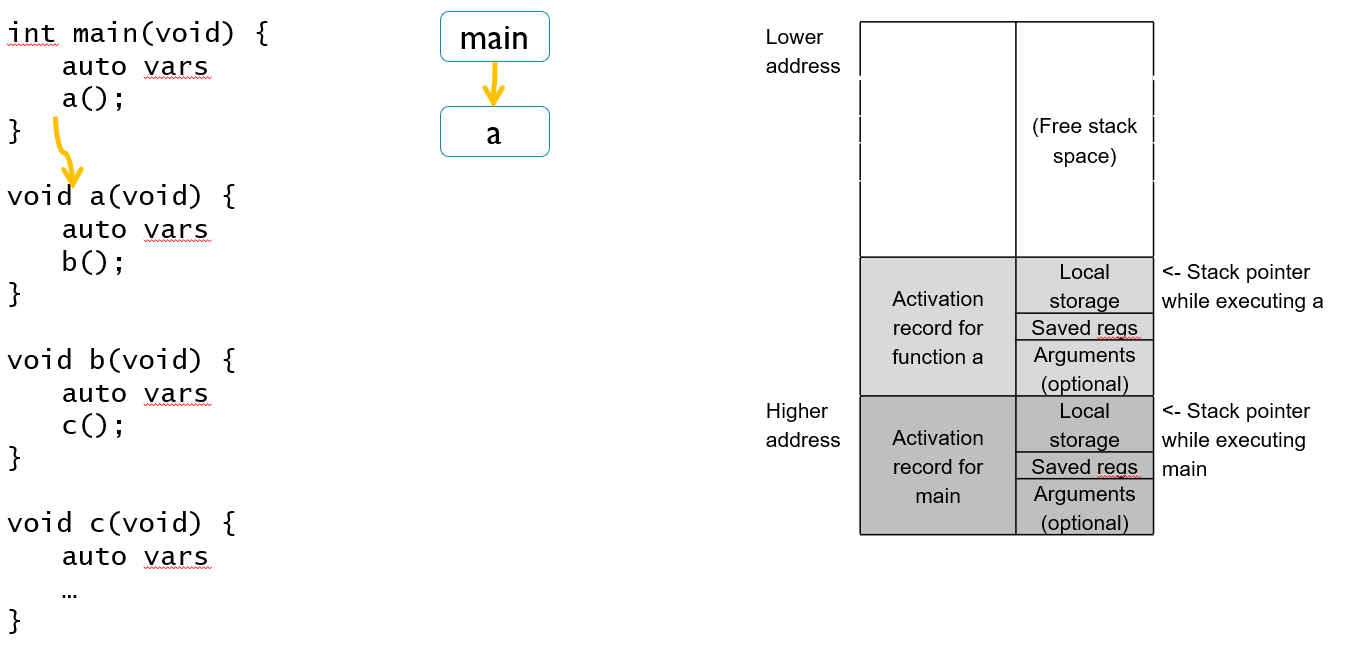
\includegraphics[scale=0.4]{StackFunction6}
	\end{figure}
\end{frame}
%%%%%%%%%%%%%%%%% FRAME %%%%%%%%%%%%%%%%%%%%%%%%%%
\begin{frame}
	\frametitle{Pila de llamado a funciones}
	\begin{figure}
		\centering
		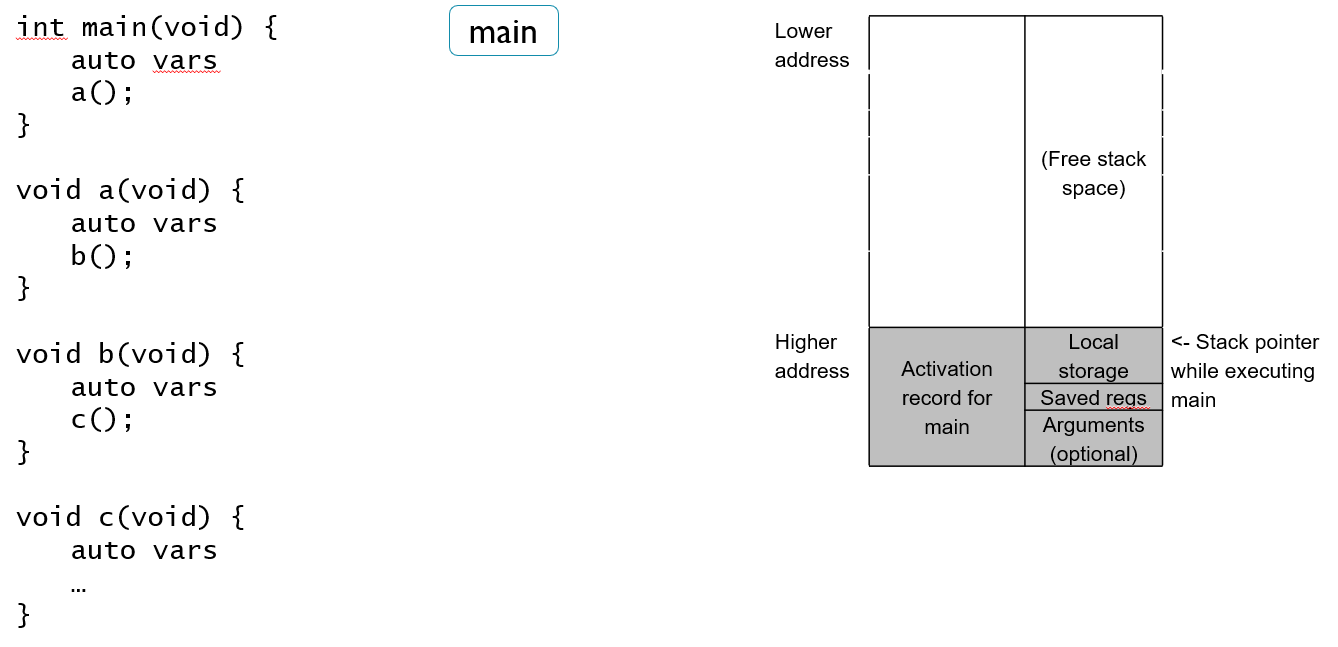
\includegraphics[scale=0.4]{StackFunction7}
	\end{figure}
\end{frame}
%%%%%%%%%%%%%%%%% FRAME %%%%%%%%%%%%%%%%%%%%%%%%%%
\begin{frame}
	\frametitle{Pila de llamado a funciones}
	\begin{figure}
		\centering
		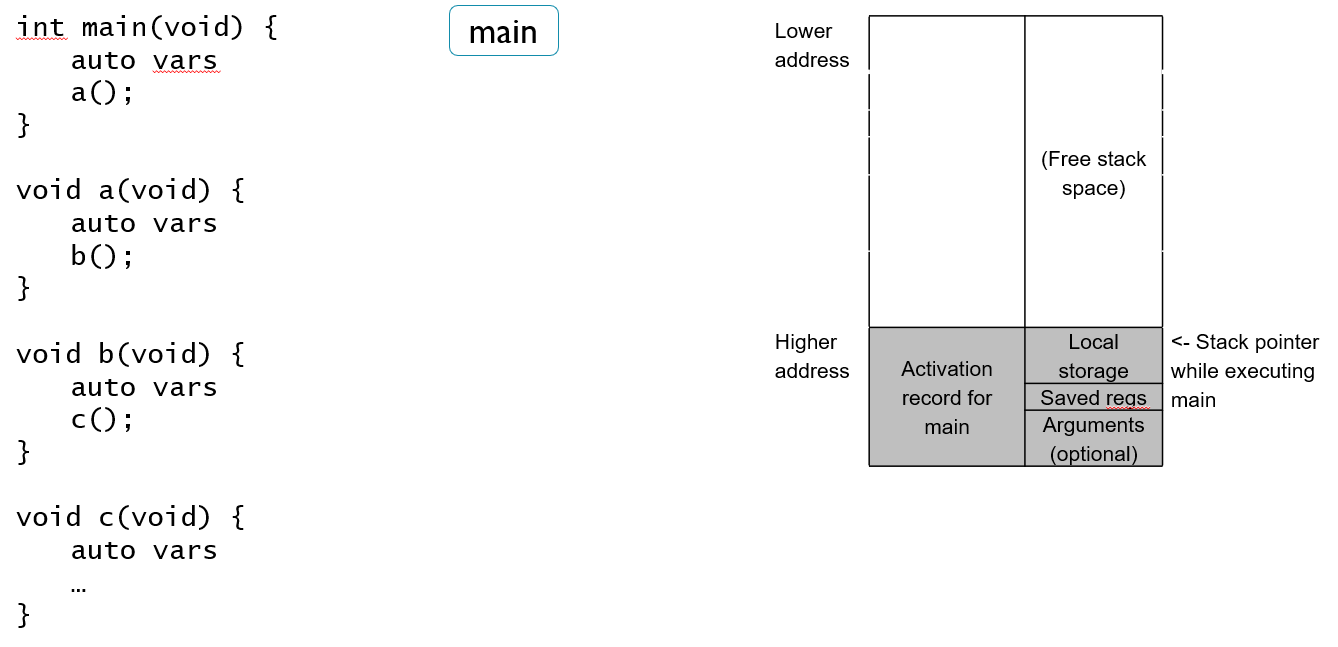
\includegraphics[scale=0.4]{StackFunction7}
	\end{figure}
\end{frame}

%%%%%%%%%%%%%%%%% FRAME %%%%%%%%%%%%%%%%%%%%%%%%%%
\begin{frame}
	\frametitle{Pila de llamado a funciones}
	\begin{columns}
		\column{0.3\linewidth}
		\begin{itemize}
			\item El stack incrementa con el llamado a subrutinas. Este desaparece una vez se ejecuten.
			\item La profundidad determina el tamaño del stack
			\item Peligro con recursividad. 
		\end{itemize}
		\column{0.7\linewidth}
		\begin{figure}
			\centering
			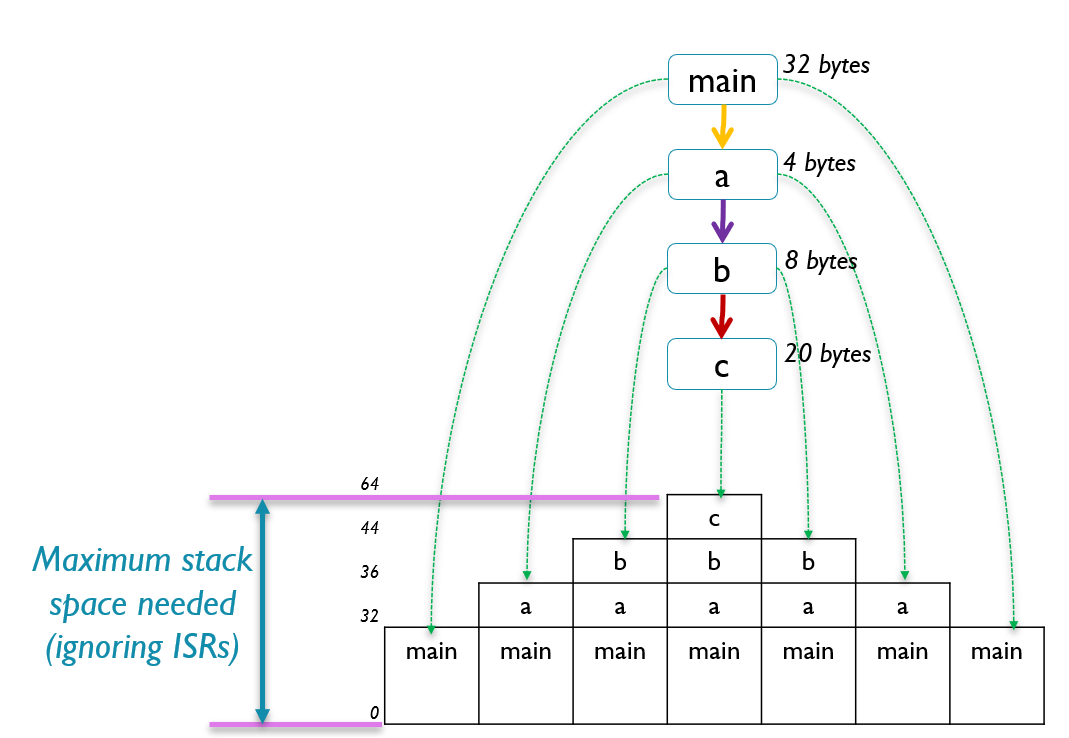
\includegraphics[scale=0.35]{MaxStack}
		\end{figure}
	\end{columns}
\end{frame}

%%%%%%%%%%%%%%%%% FRAME %%%%%%%%%%%%%%%%%%%%%%%%%%
\begin{frame}
	\frametitle{Flujo de control - If-else}
	\begin{figure}
		\centering
		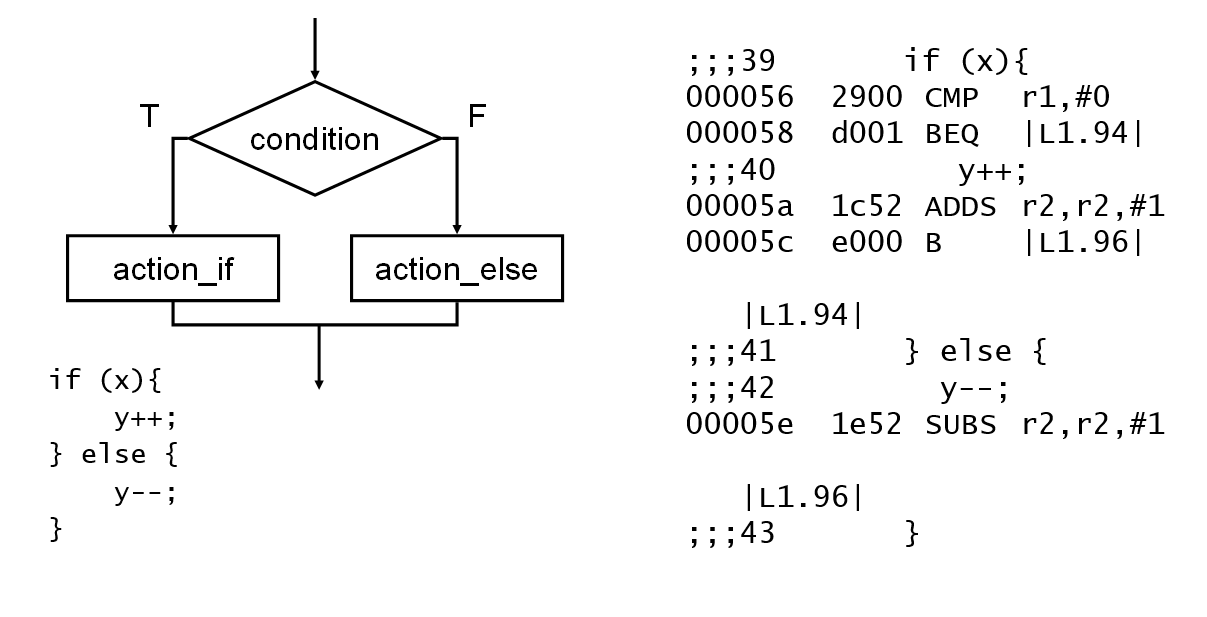
\includegraphics[scale=0.4]{IfElseAssembly}
	\end{figure}
\end{frame}

%%%%%%%%%%%%%%%%% FRAME %%%%%%%%%%%%%%%%%%%%%%%%%%
\begin{frame}
	\frametitle{Flujo de control - Switch}
	\begin{figure}
		\centering
		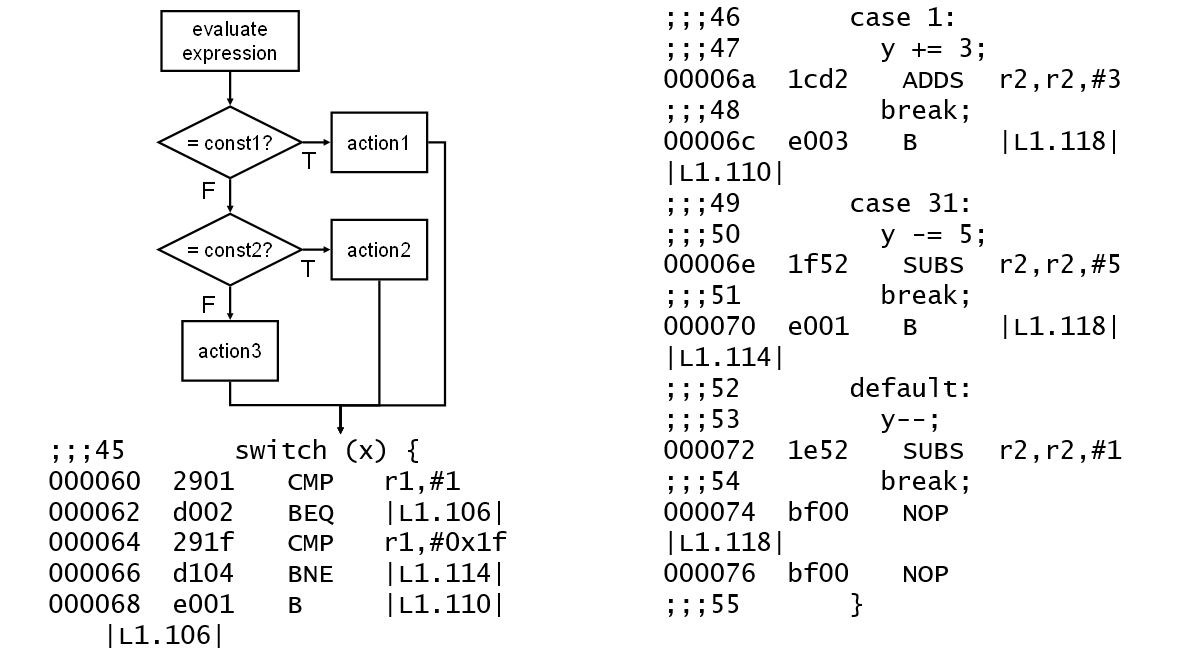
\includegraphics[scale=0.4]{SwitchAssembly}
	\end{figure}
\end{frame}
%%%%%%%%%%%%%%%%% FRAME %%%%%%%%%%%%%%%%%%%%%%%%%%
\begin{frame}
	\frametitle{Flujo de control - While}
	\begin{figure}
		\centering
		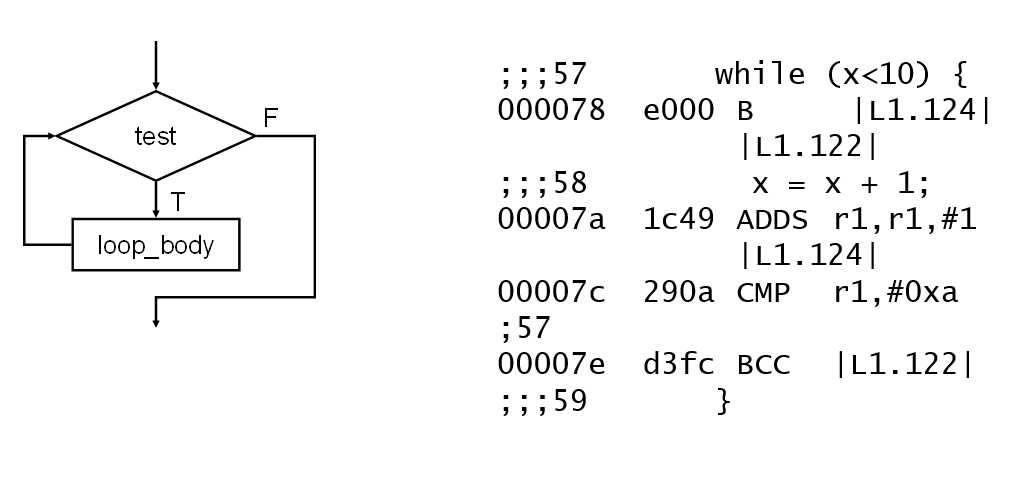
\includegraphics[scale=0.4]{WhileAssembly}
	\end{figure}
\end{frame}
%%%%%%%%%%%%%%%%% FRAME %%%%%%%%%%%%%%%%%%%%%%%%%%
\begin{frame}
	\frametitle{Flujo de control - For}
	\begin{figure}
		\centering
		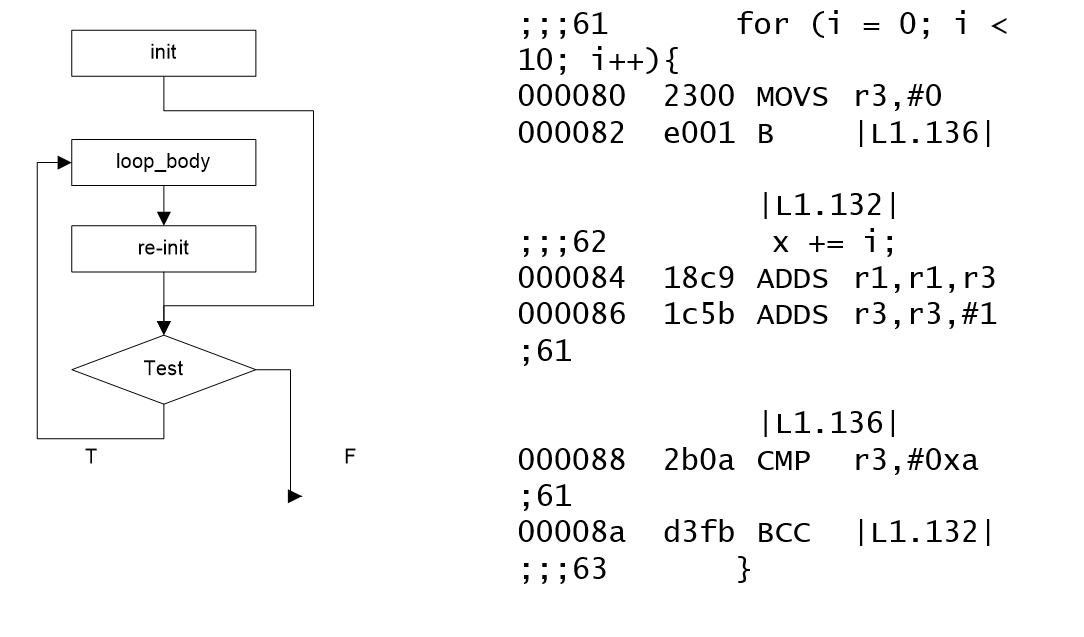
\includegraphics[scale=0.4]{ForAssembly}
	\end{figure}
\end{frame}
%%%%%%%%%%%%%%%%% FRAME %%%%%%%%%%%%%%%%%%%%%%%%%%
\begin{frame}
	\frametitle{CMSIS: Cortex Microcontroller Software Interface Standard}
	\begin{itemize}
		\item Que es CMSIS?
		\begin{itemize}
			\item Capa de abstracción de hardware: capa de software entre el programa de aplicación y el hardware. 
			\item Convenciones y estándares para la interfaz de software, estructuras y nombres.
		\end{itemize}
		\item Problemas - hay muchas opciones
		\begin{itemize}
			\item Algunas arquitecturas Cortex-M ofrecen mayores instrucciones que otras.
			\item Cuando se está trabajando con Cortex-M4, el compilador tiene instrucciones adicionales como por ejemplo operaciones de punto flotante.
			\item Muchos proveedores de MCU crean MCU basados en Cortex-M. Los procesadores son consistentes pero los perifericos cambian y su acceso a ellos de la misma forma. 
			\item Muchos compiladores disponibles. Diferentes características de optimización.
			\item Mucho RTOS disponibles.
		\end{itemize}
		\item Beneficios
		\begin{itemize}
			\item Recorta el tiempo de aprendizaje en nuevo hardware.
			\item Simplifica el desarrollo de software.
			\item Simplifica el reuso de software.
		\end{itemize}
	\end{itemize}
\end{frame}
%%%%%%%%%%%%%%%%% FRAME %%%%%%%%%%%%%%%%%%%%%%%%%%
\begin{frame}
	\frametitle{Estructura de CMSIS}
	\begin{figure}
		\centering
		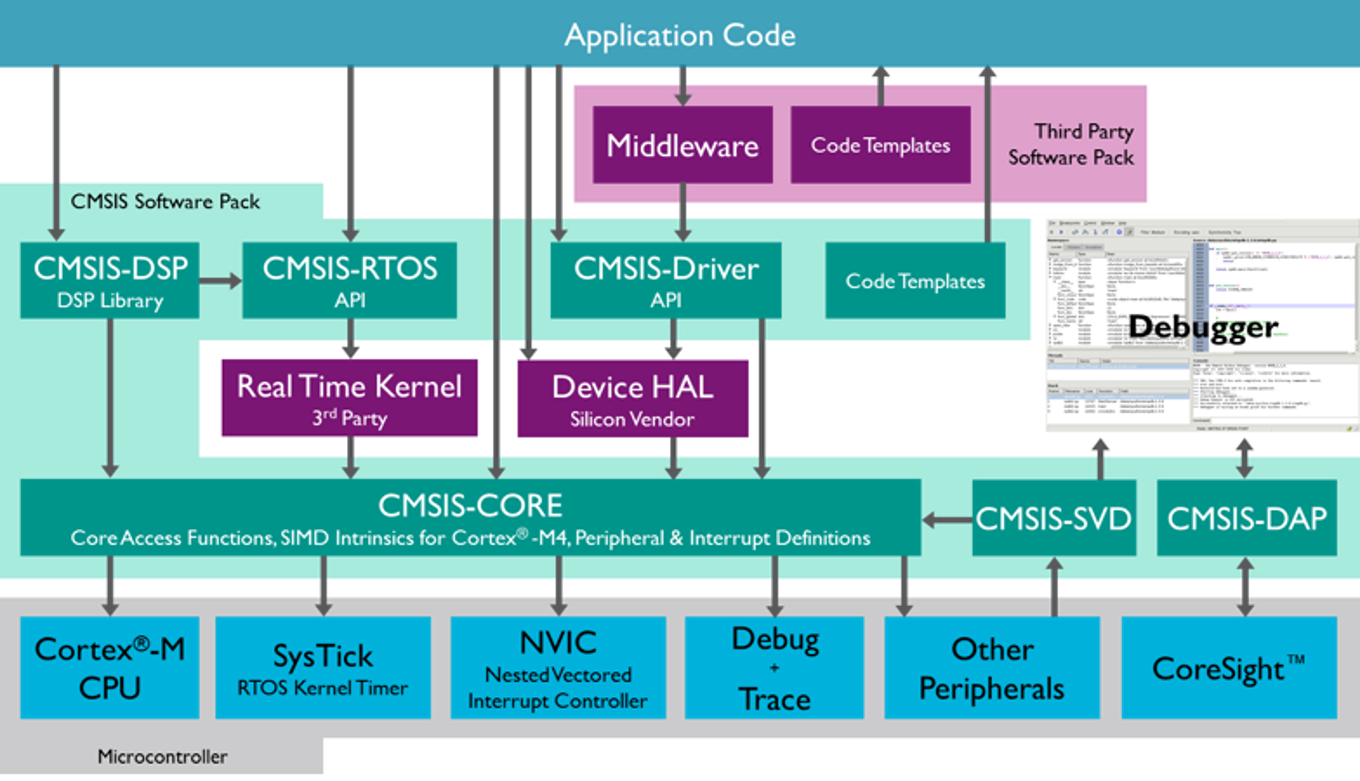
\includegraphics[scale=0.5]{CMSISStructure}
	\end{figure}
\end{frame}
%%%%%%%%%%%%%%%%% FRAME %%%%%%%%%%%%%%%%%%%%%%%%%%
\begin{frame}
	\frametitle{Convenciones de CMSIS}
	\begin{itemize}
		\item General
		\begin{itemize}
			\item Cumple con estandar ANSI C y C++
			\item Usa ANSI C $<$stdint.h$>$ para tipos de datos.
			\item Esta estructurado bajo el estándar MISRA 2004.
		\end{itemize}
		\item Convenciones para los nombres
		\begin{itemize}
			\item Nombres en mayúsculas para los registros principales, registros de periféricos, instrucciones de CPU.
			\item Minúsculas para las interrupciones y el nombre de funciones.
			\item Prefijo de espacio entre nombre '\_' para grupos.
		\end{itemize}
		\item Documentación utilizando Doxygen.
		\item Licenciamiento
		\begin{itemize}
			\item Gratis.
			\item Puede ser utilizado para todos los dispositivos Cortex-M.
		\end{itemize}
	\end{itemize}
\end{frame}
%%%%%%%%%%%%%%%%% FRAME %%%%%%%%%%%%%%%%%%%%%%%%%%
\begin{frame}
	\frametitle{CMSIS-CORE}
	\begin{figure}
		\centering
		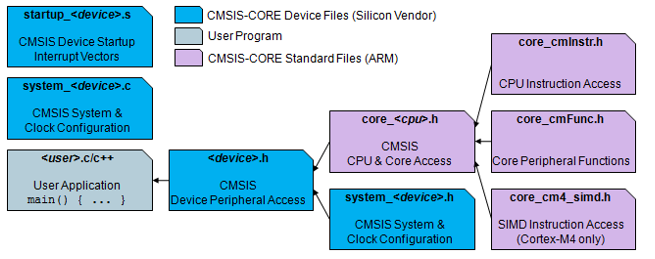
\includegraphics[scale=0.5]{CMSISCore}
	\end{figure}
	\begin{multicols}{2}
		\begin{itemize}
			\item Los archivos de dispositivo CMSIS-CORE (azul) implementan la funcionalidad específica del dispositivo
			\item La aplicación de usuario debe incluir $<$device.h$>$ para usar las funciones CMSIS-CORE. 
			\begin{itemize}
				\item Acceso a periféricos.
				\item Excepciones e interrupciones.
				\item Entre otras. 
			\end{itemize}
			\newpage
			\item Características adicionales
			\begin{itemize}
				\item API estándar para periféricos y núcleo del procesador Cortex-M
				\item Organización de archivos de encabezado y convenciones.
				\item Esqueletos de funciones de inicialización del sistema, implementados por proveedores de MCU.
				\item Soporte para determinar la frecuencia del reloj del sistema
			\end{itemize}
		\end{itemize}
	\end{multicols}
\end{frame}
%%%%%%%%%%%%%%%%% FRAME %%%%%%%%%%%%%%%%%%%%%%%%%%
\begin{frame}
	\frametitle{Registros Ejemplo}
	\begin{itemize}
		\item Archivo header MK64F12.h. 
		\begin{itemize}
			\item Este archivo define tipos de datos estructuras para acceder a los registros del sistema.
		\end{itemize} 
	\end{itemize}
	\begin{figure}
		\centering
		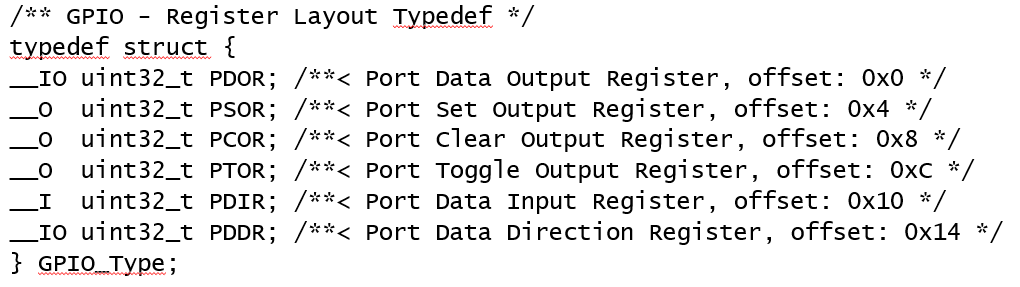
\includegraphics[scale=0.5]{GPIOStruct}
	\end{figure}
\end{frame}
%%%%%%%%%%%%%%%%% FRAME %%%%%%%%%%%%%%%%%%%%%%%%%%
\begin{frame}
	\frametitle{Registros Ejemplo}
	\begin{itemize}
		\item Archivo header MK64F12.h. 
		\begin{itemize}
			\item Declara puntero a los registros. 
		\end{itemize} 
	\end{itemize}
	\begin{figure}
		\centering
		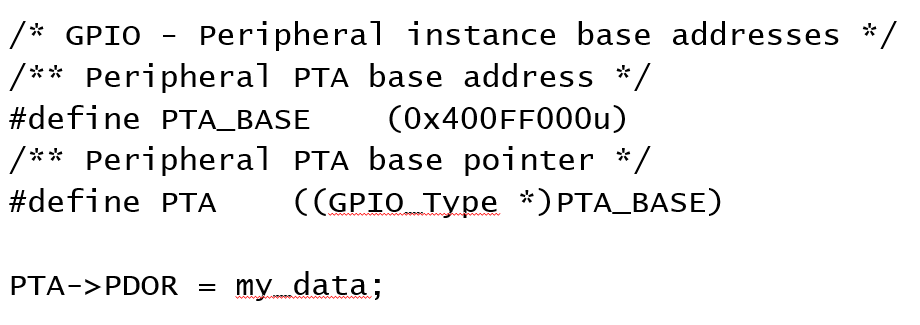
\includegraphics[scale=0.5]{GPIOPointer}
	\end{figure}
\end{frame}
%%%%%%%%%%%%%%%%% FRAME %%%%%%%%%%%%%%%%%%%%%%%%%%
\frame{
\begin{center}
	\LARGE \textcolor{blue}{INTRODUCCIÓN A LOS MICROCONTROLADORES}
\end{center}

\begin{center}
	\LARGE \textcolor{blue}{GRACIAS}
\end{center}
}

%%%%%%%%%%%%%%%%%%%%%%%%%%%%%%%%%%%%%%%%%%%%%%%%%%%%%%%%%%%%%%%%%%%%%%%%%%%%%%%%%%%%%%%%%%%%%%%%%%%%%%%%%%%%%



\end{document}

